\documentclass[a4paper]{article}

\usepackage[a4paper,top=2cm,bottom=2cm,left=3cm,right=3cm,marginparwidth=1.75cm]{geometry}
\usepackage[utf8]{inputenc}
\usepackage[T1]{fontenc}
\usepackage{textcomp}
\usepackage[ngerman]{babel}
\usepackage{amsmath, amssymb, nccmath}
\usepackage{accents}


\usepackage{multirow}
\usepackage{fancyhdr}
\usepackage{lastpage}

% figure support
\usepackage{import}
\usepackage{xifthen}
\pdfminorversion=7
\usepackage{pdfpages}
\usepackage{transparent}
\newcommand{\incfig}[1]{%
    \def\svgwidth{\columnwidth}
    \import{./figures/}{#1.pdf_tex}
}

\pdfsuppresswarningpagegroup=1

\title{Protokoll zur sechsten Laborübung\\Messtechnik Labor 376.091}
\author{DINC Atilla (11917652)}

\begin{document}
\newcommand{\unit}[1]{\ensuremath{\, \mathrm{#1}}} % Einheiten in Math-Moder richtig formatieren
% --------------------- HEADER ---------------------
\pagestyle{fancy}
% --------------------- FOOTER ---------------------
\fancyfoot[L]{Wintersemester 2023}
\fancyfoot[C]{\textbf{\thepage /\pageref{LastPage}}}
\renewcommand{\footrulewidth}{0.4pt}

\normalsize
\maketitle
\tableofcontents
\pagebreak
\section{Erklärung, Unterschrift, Allgemeines}
Alle Messungen und Ergebnisse die diesem Protokoll entstammen wurden von Atilla Dinc,
Muhammend Tesgin und Victoria Wolfgruber durchgeführt und dokumentiert.

\begin{figure}[h]
    \centering
    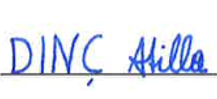
\includegraphics[width=0.3\textwidth]{images/Unterschrift}
    \caption{Unterschrift des Protokollführers DINC Atilla}
\end{figure}

\subsection{Teilnehmerinformationen}
	\begin{tabular}{|c| c|}
		\hline
        \textbf{Gruppennummer:} & 5                                                                                        \\
        \hline
		\multicolumn{2}{|c|}{\textbf{Gruppenmitglider}}                                                                                        \\
		\hline
        Name & Matrikelnummer\\
        \hline
        Atilla Dinc & 11917652\\
        Muhammed Tesgin & 12004145\\
        Victoria Wolfgruber & 11933423\\
        \hline
	\end{tabular}

\subsection{Laborausstattung}
\begin{center}
	\begin{tabular}{|c| c| c| c| c|}
		\hline
		\multicolumn{5}{|c|}{\textbf{Geräteliste}}                                                                                        \\
		\hline

		Bezeichnung              & Gerätebeschreibung                                         & Messgrößen & Inventarnummer & Bemerkungen \\
		\hline
		OZ1                      & Digitalspeicheroszilloskop DSO-x2002A                                  & -          & CD0408-7         & -           \\
		MM1                       & Digitalmultimeter                                          & -          & CA0402-1            & -           \\
		DAQ                      & CaptureCard                      & -   & CA0410-3       & -           \\
		DAC                      & DAQ-Anschluss                       & -   & CA0410-3       & -           \\
		                         & Reflektor                                          & -    & CA0410-2        & -           \\
		\hline
		\hline
		\multicolumn{5}{|c|}{\textbf{Zubehörliste}}                                                                                       \\
		\hline
		Bezeichnung              & Zubehörbeschreibung                                        & Messgrößen & Inventarnummer & Bemerkungen \\
		\hline
		RF1                       & Reflektoraufsatz & -          & -              &     -    \\
		RF2                       & Reflektoraufsatz & -          & -              &     -    \\
		\hline
	\end{tabular}
\end{center}

% ~~~~~~~~~~~~~~~~~~~~~~~~~~~~ Start of the document ~~~~~~~~~~~~~~~~~~~~~~~~~~~~

\newpage
\section{Einleitung}
In dieser Laborübung steht eine moderne Data-Aquisition-Card zur Verfügung,
welche analoge Signale über eine physikalische Schnittstelle mit BNC-Anschlüssen
einlesen und ausgeben kann. Die DA-Card dient als Schnittstelle zum Computer und
erlaubt es, mit Software-Tools wie etwa Simulink und Matlab eine digitale
Verarbeitung der Messdaten zu ermöglichen.\newline
Weiters steht Näherungssensor mit einem fein verstellbaren  Reflektor, sowie eine
Lampe zur Verfügung. Das Ziel dieser Laborübung ist es, sich dem Umgang mit der
digitalen Datenverarbeitung zu nähern indem Erfahrungen am Beispiel des
Näherungssensors gewonnen werden.

Zudem stehen mehrere Programme zur Verfügung, welche die Programmierung während
dem Labor vereinfachen sollen. Darunter sind Programme zu vorprogrammierten
Filterung der Signal, zur Kommunikation mit der DAC und auch ein Simulink-Projekt,
welches es im Laufe der Übung zu vervollständigen gilt.

\section{Aufbau zur Charakterisierung}
Zunächst wurde der Reflektor mit dem Näherungssensor für die Inbetriebnahme mit
einer Versorgungsspannung von $U_{V}=\pm12\unit{V}$ verschaltet. Der analoge
Eingang der Anschlussbox wurde mit einem T-Stück sowohl am Oszilloskop, alsauch
am Näherungssensor angeschlossen. Der Funktionsgenerator FG1 wurde mit einem T-Stück,
sowohl an Channel 2 des Oszilloskops, als auch am Eingang des Näherungssensors
angeschlossen und mit einem DC-Offset von $1,5 \unit{V}$ eingestellt.
Reflektor 1 wurde montiert und das Startup File in MatLAB wurde ausgeführt. Die
DAC konnte erfolgreich verbunden werden und der Ausgang des Näherungssensors wurde
korrekt gemessen.

\section{Aufnahme der Kennlinie}
Wie im Skriptum beschrieben, wurde das Sensorsignal mit der Abstandsabhängigkeit
aufgenommen. Dazu wurde zunächst die maximale Ausgangsspannung bestimmt, indem
der gesamte verfügbare Abstandsbereich durchfahren wurde. Wir konnte so feststellen,
dass wir nicht an die Grenzen der Ausgangsspannung geraten können und dass der
Reflektor mit dem Sensor kollidieren kann.\newline
Weiters ist uns aufgefallen, dass die Einbaumessschraube keine metrische Skala
verwendet. Unserer Vermutung nach, wird von einer imperialen Einheit ausgegangen
weshalb hier vom amerikanischen Zoll-Maß ausgegangen wird. Der Aufschrift 
der Messschraube wurde entnommen, dass die Inkrementierungen in zwölftel Zoll
Abständen voranschreiten.\newline
Für eine bessere adaptive Auflösung der stark verzerrten Kennlinie, wurde
zunächst eine grobe und im Anschluss eine feine Messung um den Höchstwert herum
durchgeführt.

\subsection{Messergebnisse}
Es konnte direkt zu Beginn festgestellt werden, dass die maximale Ausgangsspannung
des Näherungssensors nicht erreicht werden kann und dass die maximal möglich
Auslenkung der Messschraube $x_{max}=9 \frac{3}{4} \frac{1}{12}''$ beträgt.
Die grobe Messung wurde in $\frac{1}{12}''$-Schritten durchgeführt und lieferte
das Ergebnis aus Tabelle \ref{6-3-2-grobeMessung}. Daraus ist ersichtlich, dass
die sich das Maximum der Kennlinie bei einer Auslenkung von
$x_{max}\approx \frac{8}{12}''$ befindet, daher wurde die feine Aufnahme
symmetrisch um diesen Punkt herum in $\frac{1}{4}$-Inkrementierungen aufgenommen.

\begin{table}[h]
    \centering
    \caption{grobe Aufnahme der Kennlinie}
    \label{6-3-2-grobeMessung}
    \begin{tabular}{|c|c|}
        \hline
        $x \unit{[\frac{1}{12}'']}$&  $u_{mean}\unit{[V]}$ \\
        \hline
        0 & 0,06213\\
        1 & 0,06885\\
        2 & 0,08384\\
        3 & 0,1094\\
        4 & 0,1558\\
        5 & 0,2479\\
        6 & 0,4343\\
        7 & 0,7825\\
        8 & 0,9863\\
        9 & 0,3565\\
        \hline
    \end{tabular}
\end{table}

\begin{table}[h]
    \centering
    \caption{feine Aufnahme der Kennlinie}
    \label{6-3-2-feineMessung}
    \begin{tabular}{|c|c|}
        \hline
        $x \unit{[\frac{1}{12}'']}$&  $u_{mean}\unit{[V]}$ \\
        \hline
        0 & 0,06213\\
        \hline
    \end{tabular}
\end{table}
\end{document}
